\documentclass[18pt,xcolor=table]{beamer}
\usepackage{etex}
\reserveinserts{28}
\usepackage{amsmath, amssymb, amsthm, mathtools}
\usepackage{graphicx}
\usepackage{cancel}
\usepackage{color}
\usepackage{caption}
\usepackage{subcaption}
%\usepackage{subfigure}
\usepackage{pgf,tikz}
\usetikzlibrary{arrows}

\captionsetup{compatibility=false}

\newcommand{\bs}[1]{\boldsymbol{#1}}
\newcommand{\norm}[1]{\left\| #1 \right\|}
\newcommand{\snorm}[1]{\left| #1 \right|}
\newcommand{\LRp}[1]{\left( #1 \right)}
\newcommand{\LRs}[1]{\left[ #1 \right]}
\newcommand{\LRc}[1]{\left\{ #1 \right\}}
\newcommand{\LRa}[1]{\left\langle #1 \right\rangle}
\newcommand{\LRb}[1]{\left| #1 \right|}
\newcommand{\Grad}{\ensuremath{\nabla}}
\newcommand{\Gradxt}{\ensuremath{\nabla_{xt}}}
\newcommand{\Div}{\ensuremath{\nabla\cdot}}
\newcommand{\Divxt}{\ensuremath{\nabla_{xt}\cdot}}
\newcommand{\Curl}{\ensuremath{\nabla\times}}
\newcommand{\bfH}{\mbox{\boldmath $H$}}
\newcommand{\bfsigma}{\boldsymbol\sigma}
\newcommand{\bfvarsigma}{\boldsymbol\varsigma}
\newcommand{\bftau}{\boldsymbol\tau}
\newcommand{\bfbeta}{\boldsymbol\beta}
\newcommand{\bflambda}{\boldsymbol\lambda}
\newcommand{\bfpsi}{\boldsymbol\psi}
\newcommand{\bfu}{\boldsymbol u}
\newcommand{\bfv}{\boldsymbol v}
\newcommand{\bfV}{\boldsymbol V}
\newcommand{\bfZ}{\boldsymbol Z}
\newcommand{\bfz}{\boldsymbol z}
\newcommand{\bfW}{\boldsymbol W}
\newcommand{\bfw}{\boldsymbol w}
\newcommand{\bfm}{\boldsymbol m}
\newcommand{\bfM}{\boldsymbol M}
\newcommand{\bbM}{\mathbb{M}}
\newcommand{\bfq}{\boldsymbol q}
\newcommand{\bfU}{\boldsymbol U}
\newcommand{\bfS}{\boldsymbol S}
\newcommand{\bbS}{\mathbb{S}}
\newcommand{\bbD}{\mathbb{D}}
\newcommand{\bfK}{\boldsymbol K}
\newcommand{\bbK}{\mathbb{K}}
\newcommand{\bfn}{\boldsymbol n}
\newcommand{\bff}{\boldsymbol f}
\newcommand{\bfF}{\boldsymbol F}
\newcommand{\bbF}{\mathbb{F}}
\newcommand{\bfg}{\boldsymbol g}
\newcommand{\bfG}{\boldsymbol G}
\newcommand{\bfC}{\boldsymbol C}
\newcommand{\bft}{\boldsymbol t}
\newcommand{\bfT}{\boldsymbol T}
\newcommand{\bfI}{\boldsymbol I}
\newcommand{\bbI}{\mathbb{I}}
\newcommand{\bfx}{\boldsymbol x}
\newcommand{\uh}{\widehat{u}}
\newcommand{\fnh}{\widehat{f}_n}
\newcommand{\LQ}{L^2\LRp{Q}}
\newcommand{\LK}{L^2\LRp{K}}
\newcommand{\LVecK}{\mathbf{L}^2\LRp{K}}
\newcommand{\LVecQ}{\mathbf{L}^2\LRp{Q}}
\newcommand{\HdivK}{\bfH(\text{div},K)}
\newcommand{\HdivOmega}{\bfH(\text{div},\Omega)}
% \newcommand{\HdivOmegaLT}{\bfH(\text{div},\Omega)\times L^2([0,T])}
\newcommand{\HdivQ}{\bfH(\text{div}_{xt},Q)}
\newcommand{\HOneK}{H^{1}(K)}
\newcommand{\HOneVecK}{\bfH^{1}(K)}
\newcommand{\HOneQ}{H^{1}(Q)}
\newcommand{\HOneOmegah}{H^{-1}(\Omega_h)}
\newcommand{\HdivOmegah}{\bfH(\text{div},\Omega_h)}
\newcommand{\vdeltau}{v_{\delta\bs u_h}}
\newcommand{\taudeltau}{\bftau_{\delta\bs u_h}}
\newcommand{\ip}[1]{\left\langle #1 \right\rangle}
\newcommand{\pd}[2]{\frac{\partial#1}{\partial#2}}
\newcommand{\pt}[1]{\frac{\partial#1}{\partial t}}
\newcommand{\ppd}[2]{\frac{\partial^2#1}{\partial#2^2}}
\newcommand{\pdd}[3]{\frac{\partial^2#1}{\partial#2\partial#3}}
\newcommand{\der}[2]{\frac{\mathrm{d}#1}{\mathrm{d}#2}}
\newcommand{\Oh}{\Omega_h}
\newcommand{\jump}[1] {\ensuremath{\LRs{\![#1]\!}}}
\newcommand{\Gh}{\Gamma_h}
\newcommand{\mcU}{\mathcal{U}}
\newcommand{\mcUh}{\hat{\mathcal{U}}}
\newcommand{\LOmega}{L^2\LRp{\Omega_h}}

\newcommand{\eqnref}[1]{\eqref{eq:#1}}

\DeclareMathOperator*{\argmin}{arg\,min}
\DeclareMathOperator*{\trace}{tr}

\def\arrtwo#1#2#3#4{\left[
\begin{array}{cc}
#1\; & #2\\
#3\; & #4\\
\end{array}
\right]}
\def\arrthree#1#2#3#4#5#6#7#8#9{\left[
\begin{array}{ccc}
#1\; & #2\; & #3\\
#4\; & #5\; & #6\\
#7\; & #8\; & #9\\
\end{array}
\right]}
\def\arrthreeone#1#2#3{\left[
\begin{array}{ccc}
#1\; & #2\; & #3\\
\end{array}
\right]}
\def\vecttwo#1#2{\left(
\begin{array}{c}
#1\\
#2\\
\end{array}
\right)}
\def\svecttwo#1#2{\left[
\begin{array}{c}
#1\\
#2\\
\end{array}
\right]}
\def\vectthree#1#2#3{\left(
\begin{array}{c}
#1\\
#2\\
#3\\
\end{array}
\right)}
\def\svectthree#1#2#3{\left[
\begin{array}{c}
#1\\
#2\\
#3\\
\end{array}
\right]}

\renewcommand{\arraystretch}{1.2}

\def\etal{{\it et al.~}}

\graphicspath{{../PD13/figs/}{../Proposal/figs/}{../Figures/}}

\usepackage{bbm}
\usepackage{textpos}
\usepackage{pgf,tikz}
\usepackage{pgfplots}
\usepackage[space]{grffile}
\usepackage{graphicx}
\usepackage{forloop}
% \usepackage[aps,prb,citeautoscript]{revtex4-1}
% \usepackage[super]{natbib}
\usepackage[backend=bibtex,sorting=none]{biblatex}
\usepackage{animate}
\usepackage{listings}
\usepackage{bbding}
\usepackage{comment}
\usepackage{appendixnumberbeamer}
\bibliography{../Papers}

\newcounter{nn}

% \AtBeginSection[]
% {
%   \begin{frame}
%     \frametitle{Table of Contents}
%     \framesubtitle{\hspace{1ex}}
%     \tableofcontents[currentsection,currentsubsection]
%   \end{frame}
% }
% \AtBeginSubsection[] {
%   \begin{frame}
%     \frametitle{Table of Contents}
%     \framesubtitle{\hspace{1ex}}
%     \tableofcontents[currentsection,currentsubsection]
%   \end{frame}
% }

\definecolor{utorange}{RGB}{203,96,21}
\definecolor{utblack}{RGB}{99,102,106}
\definecolor{utbrown}{RGB}{110,98,89}
\definecolor{utsecbrown}{RGB}{217,200,158}
\definecolor{utsecgreen}{RGB}{208,222,187}
\definecolor{utsecblue}{RGB}{127,169,174}

\mode<presentation>
{
  % \usetheme{Pittsburgh}
  \usetheme{Boadilla}
  \usefonttheme[onlymath]{serif}

  \setbeamercovered{invisible}
  \setbeamertemplate{navigation symbols}{}

  % Color Theme
    \setbeamercolor{normal text}{bg=white,fg=utblack}
  \setbeamercolor{structure}{fg=utorange}

  \setbeamercolor{alerted text}{fg=red!85!black}

  \setbeamercolor{item projected}{use=item,fg=black,bg=item.fg!35}

  \setbeamercolor*{palette primary}{use=structure,fg=white, bg=utorange}
  \setbeamercolor*{palette secondary}{use=structure,bg=utsecbrown}
  \setbeamercolor*{palette tertiary}{use=structure,bg=utsecgreen}
  \setbeamercolor*{palette quaternary}{use=structure,fg=structure.fg,bg=utsecblue}

  % \setbeamercolor*{frametitle}{use=structure,fg=utorange, bg=utsecbrown}
  \setbeamercolor*{framesubtitle}{fg=utbrown}

  \setbeamercolor*{block title}{parent=structure,fg=black,bg=utsecgreen}
  \setbeamercolor*{block body}{fg=black,bg=utblack!10}
  \setbeamercolor*{block title alerted}{parent=alerted text,bg=black!15}
  \setbeamercolor*{block title example}{parent=example text,bg=black!15}

  \setbeamerfont{framesubtitle}{size=\small}
}

% \usepackage[orientation=landscape,size=custom,width=16,height=9.75,scale=0.5,debug]{beamerposter}
% \usepackage[orientation=landscape,size=custom,width=16,height=9,scale=0.5,debug]{beamerposter}


\makeatletter
\setbeamertemplate{footline}
{
  \leavevmode%
    \hbox{%
      \begin{beamercolorbox}[wd=.333333\paperwidth,ht=2.25ex,dp=1ex,center]{author in head/foot}%
        \usebeamerfont{author in head/foot}\insertshortauthor%~~\beamer@ifempty{\insertshortinstitute}{}{(\insertshortinstitute)}
      \end{beamercolorbox}%
        \begin{beamercolorbox}[wd=.333333\paperwidth,ht=2.25ex,dp=1ex,center]{title in head/foot}%
        \usebeamerfont{title in head/foot}\insertshorttitle
        \end{beamercolorbox}%
        \begin{beamercolorbox}[wd=.333333\paperwidth,ht=2.25ex,dp=1ex,right]{date in head/foot}%
        \usebeamerfont{date in head/foot}\insertshortdate{}\hspace*{2em}
        \insertframenumber{} / \inserttotalframenumber\hspace*{2ex}
      \end{beamercolorbox}}%
        \vskip0pt%
}
\makeatother

\usepackage{kerkis}
\usepackage[T1]{fontenc}
\usepackage[protrusion=true,expansion=true]{microtype}
\usepackage{amsmath}


\renewcommand*{\thefootnote}{\fnsymbol{footnote}}

\let\oldfootnotesize\footnotesize
\renewcommand*{\footnotesize}{\oldfootnotesize\tiny}


\pgfdeclareimage[height=1.2cm]{utbig}{logos/UTWordmark}
\pgfdeclareimage[height=0.6cm]{ut}{logos/UTWordmark}
% \pgfdeclareimage[height=10.0cm]{utbig}{logos/ICES-wordmark-teal.pdf}
% \pgfdeclareimage[height=0.6cm]{ut}{logos/ICES-wordmark-teal.pdf}
% \pgfdeclareimage[height=1.5cm]{iceslogo}{logos/ICES-wordmark-teal.png}
% \pgfdeclareimage[height=1.0cm]{scsmall}{logos/SC12}

\title[Automated Scientific Computing with DPG]{Automating Scientific Computing with Discontinuous Petrov-Galerkin Finite Elements}
% \subtitle{If you have one}
\author[Truman Everett Ellis]{ \underline{Truman~Everett~Ellis} \\[8pt]
{\oldfootnotesize \smallskip Advisors: Leszek Demkowicz, Robert Moser\\[8pt]
Committee: Thomas Hughes, Clint Dawson, Tan Bui-Thanh\\[8pt]
Collaborators: Nathan Roberts (Argonne), Jesse Chan (Virginia Tech)}
}


% \institute{Institute for Computational Engineering \& Sciences\\ \mbox{}  \\  \pgfuseimage{utbig} }
\institute{
\pgfuseimage{utbig}
\\ \vspace{2ex}

\includegraphics[trim=3.0in 7.2in 1.5in 4.0in,width=0.3\linewidth]{logos/ICES-wordmark-teal.pdf}
}
\date[April 20, 2016]%{\pgfuseimage{iceslogo} }

\begin{document}
\def\thefootnote{\arabic{footnote}}

\tikzstyle{block} = [rectangle, draw, rounded corners, shade, top color=white, text width=5em,
  bottom color=blue!50!black!20, draw=blue!40!black!60, very thick, text centered, minimum height=4em]
  \tikzstyle{line} = [draw, -latex']
  \tikzstyle{cloud} = [draw, ellipse,top color=white, bottom color=red!20, node distance=2cm, minimum height=2em]


  \beamertemplateballitem
  %\beamertemplatetransparentcoveredhigh

  \frame{\titlepage}

  \addtobeamertemplate{frametitle}{}{%
      \begin{textblock*}{100mm}(0.87\textwidth,-0.75cm)
    \pgfuseimage{ut}
    \end{textblock*}
  }

\begin{frame}
\frametitle{Table of Contents}
\framesubtitle{\hspace{1ex}}
\tableofcontents
\end{frame}

%   /$$      /$$             /$$     /$$                        /$$     /$$
%  | $$$    /$$$            | $$    |__/                       | $$    |__/
%  | $$$$  /$$$$  /$$$$$$  /$$$$$$   /$$ /$$    /$$  /$$$$$$  /$$$$$$   /$$  /$$$$$$  /$$$$$$$
%  | $$ $$/$$ $$ /$$__  $$|_  $$_/  | $$|  $$  /$$/ |____  $$|_  $$_/  | $$ /$$__  $$| $$__  $$
%  | $$  $$$| $$| $$  \ $$  | $$    | $$ \  $$/$$/   /$$$$$$$  | $$    | $$| $$  \ $$| $$  \ $$
%  | $$\  $ | $$| $$  | $$  | $$ /$$| $$  \  $$$/   /$$__  $$  | $$ /$$| $$| $$  | $$| $$  | $$
%  | $$ \/  | $$|  $$$$$$/  |  $$$$/| $$   \  $/   |  $$$$$$$  |  $$$$/| $$|  $$$$$$/| $$  | $$
%  |__/     |__/ \______/    \___/  |__/    \_/     \_______/   \___/  |__/ \______/ |__/  |__/
%
%
\section{Motivation: Automating Scientific Computing}
% ------------------------------------------------------------
\begin{frame}[t]
\frametitle{Navier-Stokes Equations}
\framesubtitle{Numerical Challenges}
\begin{columns}[c]
\begin{column}{.6\textwidth}
Robust simulation of unsteady fluid dynamics remains a challenging issue.
\vspace{2ex}

\begin{itemize}
\item{} Resolving solution features (sharp, localized viscous-scale phenomena)
\begin{itemize}
\item{} Shocks
\item{} Boundary layers - resolution needed for drag/load
\item{} Turbulence (non-localized)
\end{itemize}
% \item{} Nonlinear convergence and uniqueness of solutions
\item{} Stability of numerical schemes
\begin{itemize}
\item{} Nonlinearity
\item{} Nature of PDE changes for different flow regimes
\item{} Coarse/adaptive grids
\item{} Higher order
\end{itemize}
\end{itemize}
\end{column}
\begin{column}{.4\textwidth}
\vspace{-3ex}
\begin{figure}
\centering
\includegraphics[width=0.9\textwidth]{Motivation/bullet_shock.png}\\
Shock\\\vspace{1ex}
\includegraphics[width=0.9\textwidth]{Motivation/boundary_layer.png}\\
Boundary layer
\end{figure}
\end{column}
\end{columns}
\end{frame}


% ------------------------------------------------------------
\begin{frame}[t]
\frametitle{Motivation}
\framesubtitle{Initial Mesh Design is Expensive and Time-Consuming}
\begin{columns}[t]
\begin{column}[c]{0.4\textwidth}
\begin{itemize}
  \item Surface mesh must accurately represent geometry
  \item Volume mesh needs sufficient resolution for asymptotic regime
  % Before we accurately know the flow features
  % \item Boundary layer meshes must respect $y^+$ guidelines
  \item Engineers often forced to work by trial and error
  \item Bad in the context of HPC
  \uncover<2>{\item \textcolor{utorange}{We desire an automated computational technology}}
\end{itemize}
\end{column}
\begin{column}[c]{0.6\textwidth}
\vspace{2ex}
\begin{figure}[t]
\centering
\includegraphics[width=1.0\textwidth]{Motivation/NumecaRaceCar.png}
\\\small{Formula 1 Mesh by Numeca}\\
\end{figure}
\end{column}
\end{columns}
\end{frame}


% ------------------------------------------------------------
\begin{frame}[t]
\frametitle{DPG on Coarse Meshes}
\framesubtitle{Adaptive Solve of the Carter Plate Problem\footfullcite{JesseDissertation} $Re=1000$}
\begin{columns}
\begin{column}{0.49\textwidth}
\begin{figure}
\centering
\includegraphics[width=1.0\textwidth]{Motivation/PlateMovie/T0.png}\\
\vspace{-1ex}
{\scriptsize Temperature on Initial Mesh}\\
\vspace{1ex}
\includegraphics[width=1.0\textwidth]{Motivation/PlateMovie/T8.png}
\vspace{-1ex}
{\scriptsize Temperature after 8 Refinements}
\vspace{1ex}

\end{figure}
\end{column}
\begin{column}{0.49\textwidth}
\begin{figure}
\centering
\includegraphics[width=1.0\textwidth]{Motivation/PlateMovie/T4.png}\\
\vspace{-1ex}
{\scriptsize Temperature after 4 Refinements}\\
\vspace{1ex}
\includegraphics[width=1.0\textwidth]{Motivation/PlateMovie/T11.png}
\vspace{-1ex}
{\scriptsize Temperature after 11 Refinements}
\vspace{1ex}
\end{figure}
\end{column}
\end{columns}
% \foreach \n in {1,...,11}
% {
% \only<\n>
% {
% \begin{figure}[ht]
% \centering
% \begin{subfigure}[c]{0.45\textwidth}
% \centering
% \includegraphics[width=0.99\textwidth]{Motivation/Plate/u\n.png}\\
% \vspace{-1ex}
% {\scriptsize Velocity}\\
% \end{subfigure}
% \begin{subfigure}[c]{0.45\textwidth}
% \centering
% \includegraphics[width=0.99\textwidth]{Motivation/Plate/T\n.png}\\
% \vspace{-1ex}
% {\scriptsize Temperature}\\
% \end{subfigure}
% \begin{subfigure}[c]{0.5\textwidth}
% \centering
% \vspace{2ex}
% \includegraphics[width=0.99\textwidth]{Motivation/Plate/mesh\n.png}\\
% \vspace{-1ex}
% {\scriptsize Mesh \n}\\
% \end{subfigure}
% \end{figure}
% }
% }
\end{frame}

\begin{frame}[t]
\frametitle{Lessons from Other Methods}
\framesubtitle{~~}
\begin{description}
  \item[Streamline Upwind Petrov-Galerkin:] Adaptively changing the test space can produce a method with better stability.
  \item[Discontinuous Galerkin:] Discontinuous basis functions are a legitimate option for finite element methods.
  \item[Hybridized DG:] Mesh interface unknowns can facilitate static condensation -- reducing the number of DOFs in the global solve.
  \item[Least-Squares FEM:] The finite element method is most powerful in a minimum residual context (i.e. as a Ritz method).
  \item[Space-Time FEM:] Highly adaptive methods should have adaptive time integration.
  Superior framework for problems with moving boundaries.
  Requires a method that is both temporally and spatially stable.
  % \item[Mixed FEM:] A first order formulation gives more flexibility.
\end{description}
% SUPG - changing your test space can produce better stability.

% DG - Discontinuous basis functions are a legitimate option in the finite element framework.

% HDG - Mesh interface unknowns can facilitate static condensation -- reducing the number of DOFs in the global solve.

% Least Squares

% Space-Time FEM -
%   \item Satisfies geometric conservation laws\footnotemark
%   \item Tezduyar \etal\footnotemark developed a Galerkin/least-squares method for moving boundaries
\end{frame}

%   /$$       /$$   /$$           /$$$$$$$                       /$$
%  | $$      |__/  | $$          | $$__  $$                     |__/
%  | $$       /$$ /$$$$$$        | $$  \ $$  /$$$$$$  /$$    /$$ /$$  /$$$$$$  /$$  /$$  /$$
%  | $$      | $$|_  $$_/        | $$$$$$$/ /$$__  $$|  $$  /$$/| $$ /$$__  $$| $$ | $$ | $$
%  | $$      | $$  | $$          | $$__  $$| $$$$$$$$ \  $$/$$/ | $$| $$$$$$$$| $$ | $$ | $$
%  | $$      | $$  | $$ /$$      | $$  \ $$| $$_____/  \  $$$/  | $$| $$_____/| $$ | $$ | $$
%  | $$$$$$$$| $$  |  $$$$/      | $$  | $$|  $$$$$$$   \  $/   | $$|  $$$$$$$|  $$$$$/$$$$/
%  |________/|__/   \___/        |__/  |__/ \_______/    \_/    |__/ \_______/ \_____/\___/
%
%
%
% \subsection{Literature Review}
% % ------------------------------------------------------------
% \begin{frame}[t]
% \frametitle{Stabilized Finite Elements for CFD}
% \framesubtitle{Streamline Upwind Petrov-Galerkin}
% \begin{columns}[c]
% \begin{column}{.65\textwidth}
% \begin{itemize}
%   \item First successful finite element method for CFD\footnotemark
%   \item Residual based stabilization preserves consistency
%   \item Upwind biasing of test functions
%   \item Higher order generalizations possible
%   \item Optimal $H_0^1$ approximation in 1D
%   \item Gave rise to the field of stabilized finite elements
%   \item Major contributors include Hughes, Franca, Johnson, Codina, Tezduyar, and many others
%   \item Variational multiscale may be considered the spiritual successor to SUPG\footnotemark
% \end{itemize}
% \end{column}
% \footnotetext[2]{\fullcite{SUPG}}
% \footnotetext[3]{\fullcite{VMS}}
% \begin{column}{.35\textwidth}
% \begin{figure}[t]
% \centering
% \includegraphics[width=1.0\textwidth]{Motivation/SUPG.png}
% \\\small{$H_0^1$ Projection}\\
% \end{figure}
% \end{column}
% \end{columns}
% \end{frame}


% % ------------------------------------------------------------
% \begin{frame}[t]
% \frametitle{Streamline Upwind Petrov-Galerkin}
% \framesubtitle{Two Equivalent Views on Stabilization}
% Convection-diffusion can be written as
% $$
% Lu=(L_{adv}+L_{diff})u=f\,.
% $$\\
% % Two equivalent views on stabilization.
% \vspace{-3ex}
% \begin{columns}[t]
% \begin{column}{.65\textwidth}
% \begin{block}{Residual Based Stabilization}
% \[
% b_{SUPG}(u,v)=l_{SUPG}(v)
% \]
% where
% \begin{align*}
%   b_{SUPG}(u,v)&=b(u,v)
%   +\sum_K\int_K\tau(L_{adv}v)(Lu-f)\\
%   l_{SUPG}(v)&=l(v)+\sum_K\int_K\tau(L_{adv}v)f\,,
% \end{align*}
% $\tau$ is the SUPG stabilization parameter.
% \end{block}
% \end{column}
% \begin{column}{.33\textwidth}
% \begin{block}{Test Space Modification}
% \[
% b(u,\tilde v)=l(\tilde v)
% \]
% where
% \[
% \tilde v = v+\tau L_{adv}v\,.
% \]
% \includegraphics[width=1.0\textwidth]{Motivation/SUPGtest.png}
% \end{block}
% \end{column}
% \end{columns}
% \medskip
% \end{frame}


% % ------------------------------------------------------------
% \begin{frame}[t]
% \frametitle{Stabilized Finite Elements for CFD}
% \framesubtitle{Discontinuous Galerkin}
% \begin{itemize}
%   \item Combines elements of finite volumes and finite elements
%   \item First proposed for neutron transport\footfullcite{ReedHillDG}
%   \item Early contributors include Babu\v{s}ka, Lions, Nitsche, and Zl\'{a}mal
%   \item Develoment for CFD by Cockburn and Shu\footfullcite{CockburnShuDG}
%   \item Development for elliptic problems given by Arnold, Brezzi, Cockburn, and Marini\footfullcite{ArnoldDG}
%   % \item Rigorous mathematical foundation of finite elements
%   \item Nonconforming basis, locally conservative
%   \item Naturally high order, but may require additional stabilization
%   % \item Simple to parallelize
%   \item Other notable contributors include Peraire, Persson, Karniadakis \dots
% \end{itemize}
% \end{frame}


% % ------------------------------------------------------------
% \begin{frame}[t]
% \frametitle{Stabilized Finite Elements for CFD}
% \framesubtitle{Discontinuous Galerkin}
% Consider 1D convection equation
% \[
% \pd{\beta(x)u}{x}=f,\quad u(0)=u_0\,.
% \]
% Multiply by test function and integrate by parts over each element $K=[x_K,x_{x+1}]$
% \[
% -\int_K\beta(x)u\pd{v}{x}+\beta uv|_{x_K}^{x_{K+1}}=\int_K fv\,.
% \]
% Apply upwind flux
% \[
% -\int_K\beta(x)u\pd{v}{x}+\beta(x_{K+1})u(x_{K+1}^-)v(x_{K+1}^-)-\beta(x_K)u(x_K^-)v(x_K^+)=\int_K fv\,.
% \]
% Hybridized DG (HDG) method introduces trace unknowns which facilitates static condensation, reducing interface unknowns\footfullcite{HDG}.
% \end{frame}

% % ------------------------------------------------------------
% \begin{frame}[t]
% \frametitle{Space-Time Finite Element Methods}
% \framesubtitle{Treat Time as Another Dimension to be Discretized}
% Space-time methods treat time as just another dimension to be discretized.
% \begin{columns}[c]
% \begin{column}{.7\textwidth}
% \begin{itemize}
%   \item Early contributors include Kaczkowski and Oden
%   \item Satisfies geometric conservation laws\footnotemark
%   \item Tezduyar \etal\footnotemark developed a Galerkin/least-squares method for moving boundaries
%   % deforming-spatial-domain/space-time procedure
%   % with Galerkin/least-squares to handle moving domains with incompressible and compressible flow
%   \item Van der Vegt and Van der Ven developed a popular space-time DG method\footnotemark
%   \item {\"U}ng{\"o}r's tent-pitcher algorithm\footnotemark decouples space-time elements
% \end{itemize}
% \end{column}
% \footnotetext[8]{\fullcite{GCL}}
% \footnotetext[9]{\fullcite{Tezduyar1992}}
% \footnotetext[10]{\fullcite{vanderVegtEuler}}
% \footnotetext[11]{\fullcite{TentPitcher}}
% \begin{column}{.3\textwidth}
% \includegraphics[width=1.0\textwidth]{Motivation/TentPitcher.png}
% \end{column}
% \end{columns}
% \end{frame}



%   /$$$$$$$  /$$$$$$$   /$$$$$$         /$$$$$$                                            /$$
%  | $$__  $$| $$__  $$ /$$__  $$       /$$__  $$                                          |__/
%  | $$  \ $$| $$  \ $$| $$  \__/      | $$  \ $$ /$$    /$$  /$$$$$$   /$$$$$$  /$$    /$$ /$$  /$$$$$$  /$$  /$$  /$$
%  | $$  | $$| $$$$$$$/| $$ /$$$$      | $$  | $$|  $$  /$$/ /$$__  $$ /$$__  $$|  $$  /$$/| $$ /$$__  $$| $$ | $$ | $$
%  | $$  | $$| $$____/ | $$|_  $$      | $$  | $$ \  $$/$$/ | $$$$$$$$| $$  \__/ \  $$/$$/ | $$| $$$$$$$$| $$ | $$ | $$
%  | $$  | $$| $$      | $$  \ $$      | $$  | $$  \  $$$/  | $$_____/| $$        \  $$$/  | $$| $$_____/| $$ | $$ | $$
%  | $$$$$$$/| $$      |  $$$$$$/      |  $$$$$$/   \  $/   |  $$$$$$$| $$         \  $/   | $$|  $$$$$$$|  $$$$$/$$$$/
%  |_______/ |__/       \______/        \______/     \_/     \_______/|__/          \_/    |__/ \_______/ \_____/\___/
%
%
%
\section{DPG: A Framework for Computational Mechanics}
% ------------------------------------------------------------
\begin{frame}[t]
\frametitle{Overview of DPG}
\framesubtitle{DPG is a Minimum Residual Method}
Find $u\in U$ such that
\[
b(u,v)=l(v)\quad\forall v\in V
\]
with operator $B:U\rightarrow V'$ defined by $b(u,v)=\LRa{Bu,v}_{V'\times V}$.

This gives the operator equation
\[
Bu=l\quad\in V'\,.
\]
We wish to minimize the residual $Bu-l\in V'$:
\[
u_h=\argmin_{w_h\in U_h}\frac{1}{2}\norm{Bw_h-l}^2_{V'}\,.
\]
Dual norms are not computationally tractable.
Inverse Riesz map moves the residual to a more accessible space:
\[
u_h=\argmin_{w_h\in U_h}\frac{1}{2}\norm{R_V^{-1}(Bw_h-l)}^2_{V}\,.
\]
\end{frame}


% ------------------------------------------------------------
\begin{frame}[t]
\frametitle{Overview of DPG}
\framesubtitle{Petrov-Galerkin with Optimal Test Functions}
% \framesubtitle{Optimal Petrov-Galerkin Methods}
Taking the G\^ateaux derivative to be zero in all directions $\delta u \in
U_h$ gives,
\[
\left(R_V^{-1}(Bu_h-l),R_V^{-1}B\delta u\right)_V = 0, \quad \forall \delta u \in U,
\]
which by definition of the Riesz map is equivalent to
\begin{equation*}
\LRa{Bu_h-l,R_V^{-1}B\delta u_h}=0\quad\forall\delta u_h\in U_h\,,
\end{equation*}
with optimal test functions $v_{\delta u_h}\coloneqq R_V^{-1}B\delta u_h$ for each trial function $\delta u_h$.
\begin{block}{Resulting Petrov-Galerkin System}
This gives a simple bilinear form
\begin{equation*}
b(u_h,v_{\delta u_h})=l(v_{\delta u_h}),
\end{equation*}
with $v_{\delta u_h}\in V$ that solves the auxiliary problem
\begin{equation*}
\LRp{v_{\delta u_h},\delta v}_V=\LRa{R_Vv_{\delta u_h},\delta v}
=\LRa{B\delta u_h,\delta v}=b(\delta u_h,\delta v)\quad\forall\delta v\in V.
\end{equation*}
\end{block}
\end{frame}




%    /$$$$$$                                                  /$$$$$$$$ /$$
%   /$$__  $$                                                |__  $$__/|__/
%  | $$  \__/  /$$$$$$   /$$$$$$   /$$$$$$$  /$$$$$$            | $$    /$$ /$$$$$$/$$$$   /$$$$$$
%  |  $$$$$$  /$$__  $$ |____  $$ /$$_____/ /$$__  $$ /$$$$$$   | $$   | $$| $$_  $$_  $$ /$$__  $$
%   \____  $$| $$  \ $$  /$$$$$$$| $$      | $$$$$$$$|______/   | $$   | $$| $$ \ $$ \ $$| $$$$$$$$
%   /$$  \ $$| $$  | $$ /$$__  $$| $$      | $$_____/           | $$   | $$| $$ | $$ | $$| $$_____/
%  |  $$$$$$/| $$$$$$$/|  $$$$$$$|  $$$$$$$|  $$$$$$$           | $$   | $$| $$ | $$ | $$|  $$$$$$$
%   \______/ | $$____/  \_______/ \_______/ \_______/           |__/   |__/|__/ |__/ |__/ \_______/
%            | $$
%            | $$
%            |__/


\section{Space-Time Convection-Diffusion}
% ------------------------------------------------------------
\begin{frame}[t]
\frametitle{Space-Time DPG}
\framesubtitle{Extending DPG to Transient Problems}
\begin{itemize}
  \item Time stepping techniques are not ideally suited to highly adaptive grids
  \item Space-time FEM proposed as a solution
  \begin{itemize}
    \item[\textcolor{green}{\Checkmark}] Unified treatment of space and time
    \item[\textcolor{green}{\Checkmark}] Local space-time adaptivity (local time stepping)
    \item[\textcolor{green}{\Checkmark}] Parallel-in-time integration (space-time multigrid)
    \item[\XSolidBrush] Spatially stable FEM methods may not be stable in space-time
    \item[\XSolidBrush] Need to support higher dimensional problems
  \end{itemize}
  \item DPG provides necessary stability and adaptivity
\end{itemize}
\begin{figure}[b]
\centering
\includegraphics[width=0.8\textwidth]{Schematics/XBraid}
\\
Courtesy of XBraid by LLNL
\end{figure}
\end{frame}


% ------------------------------------------------------------
\begin{frame}[t]
\frametitle{Space-Time DPG for Convection-Diffusion}
\framesubtitle{Space-Time Divergence Form}
Equation is parabolic in space-time.
\[
\pd{u}{t}+\bfbeta\cdot\Grad u-\epsilon\Delta u=f
\]
This is just a composition of a constitutive law and conservation of mass.
\begin{align*}
\bfsigma-\epsilon\Grad u&=0\\
\pd{u}{t}+\Div\LRp{\bfbeta u-\bfsigma}&=f
\end{align*}

We can rewrite this in terms of a space-time divergence.
\begin{align*}
\frac{1}{\epsilon}\bfsigma-\Grad u &=0\\
\Gradxt\cdot\vecttwo{\bfbeta u-\bfsigma}{u}&=f
\end{align*}
\end{frame}


% ------------------------------------------------------------
\begin{frame}[t]
\frametitle{Space-Time DPG for Convection-Diffusion}
\framesubtitle{Ultra-Weak Formulation with Discontinuous Test Functions}  %% needed for proper positioning of the logo ...
% \vspace{-2ex}
Multiply by test function and integrate by parts over space-time element K.
\begin{equation*}
\begin{aligned}
\LRp{\frac{1}{\epsilon}\bfsigma,\bftau}_K+\LRp{u,\Div\bftau}_K-\LRa{\hat u,\bftau\cdot\bfn_x}_{\partial K}&=0\\
-\LRp{\vecttwo{\bfbeta u-\bfsigma}{u},\Gradxt v}_K+\LRa{\hat t,v}_{\partial K}&=f
\end{aligned}
\end{equation*}
\begin{columns}[t] % contents are top vertically aligned
\begin{column}[T]{0.4\textwidth} % each column can also be its own environment
\vspace{-3ex}
where
\vspace{-1ex}
\begin{align*}
\hat u&:=\trace(u)\\
\hat t&:=\trace(\bfbeta u-\bfsigma)\cdot\bfn_x\\
&+\trace(u)\cdot n_t
\end{align*}
\vspace{-4ex}
\begin{itemize}
  \item Trace $\hat u$ defined on spatial boundaries
  \item Flux $\hat t$ defined on all boundaries
\end{itemize}
\end{column}
\begin{column}[T]{0.6\textwidth} % alternative top-align that's better for graphics
\vspace{-2ex}
\begin{block}{Support of Trace Variables}
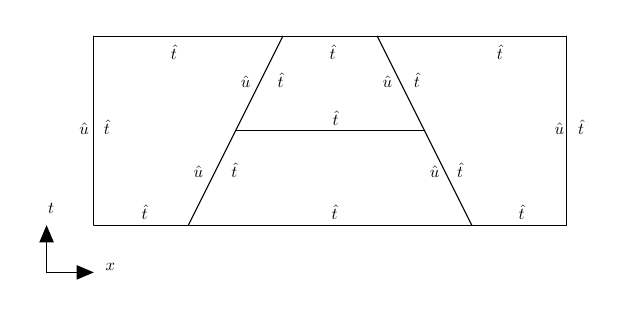
\begin{tikzpicture}[line cap=round,line join=round,>=triangle 45,x=2.0cm,y=2.0cm, scale=0.6, every node/.style={scale=0.6}]
\clip(-0.7,-0.6) rectangle (5.27,2.09);
\draw (0,2)-- (0,0);
\draw (0,0)-- (1,0);
\draw (1,0)-- (4,0);
\draw (4,0)-- (5,0);
\draw (5,0)-- (5,2);
\draw (5,2)-- (3,2);
\draw (3,2)-- (2,2);
\draw (2,2)-- (0,2);
\draw (1,0)-- (1.5,1);
\draw (1.5,1)-- (2,2);
\draw (1.5,1)-- (3.5,1);
\draw (3,2)-- (3.5,1);
\draw (3.5,1)-- (4,0);
\draw (-0.21,0.9) node[anchor=south west] {$\hat u$};
\draw (4.82,0.9) node[anchor=south west] {$\hat u$};
\draw (3.5,0.45) node[anchor=south west] {$\hat u$};
\draw (1.0,0.45) node[anchor=south west] {$\hat u$};
\draw (1.5,1.4) node[anchor=south west] {$\hat u$};
\draw (3.0,1.4) node[anchor=south west] {$\hat u$};
\draw (0.05,0.9) node[anchor=south west] {$\hat t$};
\draw (1.40,0.45) node[anchor=south west] {$\hat t$};
\draw (3.79,0.45) node[anchor=south west] {$\hat t$};
\draw (2.47,1.0) node[anchor=south west] {$\hat t$};
\draw (3.33,1.4) node[anchor=south west] {$\hat t$};
\draw (1.89,1.4) node[anchor=south west] {$\hat t$};
\draw (5.07,0.9) node[anchor=south west] {$\hat t$};
\draw (4.44,0.0) node[anchor=south west] {$\hat t$};
\draw (2.46,0.0) node[anchor=south west] {$\hat t$};
\draw (0.45,0.0) node[anchor=south west] {$\hat t$};
\draw (2.44,1.7) node[anchor=south west] {$\hat t$};
\draw (0.76,1.7) node[anchor=south west] {$\hat t$};
\draw (4.21,1.7) node[anchor=south west] {$\hat t$};
\draw [->] (-0.5,-0.5) -- (-0.5,0);
\draw [->] (-0.5,-0.5) -- (0,-0.5);
\draw (-0.54,0.29) node[anchor=north west] {$t$};
\draw (0.07,-0.35) node[anchor=north west] {$x$};
\end{tikzpicture}
\end{block}
\end{column}
\end{columns}
\end{frame}





\section{Space-Time Compressible Navier-Stokes}
% ------------------------------------------------------------
\begin{frame}[t]
\frametitle{Space-Time Compressible Navier-Stokes}
\framesubtitle{First Order System with Primitive Variables}
Assuming Stokes hypothesis, ideal gas law, and constant viscosity:
\begin{align*}
  \frac{1}{\mu}\mathbb{D}-\Grad\bfu&=0\\
  \frac{Pr}{C_p\mu}\bfq+\Grad T&=0\\
  \Divxt\vecttwo{\rho\bfu}{\rho}&=f_c\\
  \Divxt\vecttwo{\rho\bfu\otimes\bfu+\rho RT\bbI-\LRp{\bbD+\bbD^T-\frac{2}{3}\trace(\bbD)\bbI}}{\rho\bfu}&=\bff_m\\
  \Divxt\vecttwo{\rho\bfu\LRp{C_v T+\frac{1}{2}\bfu\cdot\bfu}+\rho RT\bfu+\bfq-\bfu\cdot\LRp{\bbD+\bbD^T-\frac{2}{3}\trace(\bbD)\bbI}}{\rho\LRp{C_v T+\frac{1}{2}\bfu\cdot\bfu}}&=f_e
\end{align*}
\end{frame}


% ------------------------------------------------------------
\begin{frame}[t]
\frametitle{Space-Time Compressible Navier-Stokes}
\framesubtitle{Compact Notation}
\begin{columns}[t]
\begin{column}{0.5\textwidth}
Conserved quantities
\vspace{-2ex}
\begin{align*}
C_c&:=\rho\\
\bfC_m&:=\rho\bfu\\
C_e&:=\rho(C_v T+\frac{1}{2}\bfu\cdot\bfu)\\
% C&:=\LRc{C_c\,,\, \bfC_m\,,\, C_e}\\
\end{align*}
\end{column}
\begin{column}{0.5\textwidth}
Euler fluxes
\vspace{-2ex}
\begin{align*}
\bfF_c&:=\rho\bfu\\
\bbF_m&:=\rho\bfu\otimes\bfu+\rho RT\bbI\\
\bfF_e&:=\rho\bfu\LRp{C_v T+\frac{1}{2}\bfu\cdot\bfu}+\rho RT\bfu\\
% F&:=\LRc{\bfF_c\,,\, \bbF_m\,,\, \bfF_e}\\
\end{align*}
\end{column}
\end{columns}
\begin{columns}[t]
\begin{column}{0.3\textwidth}
Viscous fluxes
\vspace{-2ex}
\begin{align*}
\bfK_c&:=\boldsymbol 0\\
\bbK_m&:=\bbD+\bbD^T-\frac{2}{3}\trace(\bbD)\bbI\\
\bfK_e&:=-\bfq+\bfu\cdot\LRp{\bbD+\bbD^T-\frac{2}{3}\trace(\bbD)\bbI}\\
% K&:=\LRc{\bfK_c\,,\, \bbK_m\,,\, \bfK_e}\\
\end{align*}
\end{column}
\begin{column}{0.3\textwidth}
Viscous variables
\vspace{-2ex}
\begin{align*}
\bbM_{\bbD}&:=\bbD\\
\bfM_{\bfq}&:=\frac{Pr}{C_p}\bfq\\
% M&:=\LRc{\bbM_{\bbD}\,,\, \bfM_{\bfq}}\\
\bfG_{\bbD}&:=2\bfu\\
G_{\bfq}&:=-T\\
% G&:=\LRc{\bfG_{\bbD}\,,\, G_{\bfq}}\\
\end{align*}
\end{column}
\end{columns}
\centering
% \begin{align*}
% f&:=\LRc{f_c\,,\, \bff_m\,,\, f_e}\\
% \end{align*}
% and group variables
% \begin{align*}
% W&:=\LRc{\rho\,,\,\bfu\,,\,T}\\
% \hat W&:=\LRc{2\hat\bfu\,,\,-\hat T}\\
% \Sigma&:=\LRc{\bbD,\bfq}\\
% \hat t&:=\LRc{\hat t_e\,,\,\hat\bft_m,\,,\,\hat t_e}\\
% \Psi&:=\LRc{\bbS\,,\,\bftau}\\
% V&:=\LRc{v_c\,,\,\bfv_m,\,,\,v_e}\,.
% \end{align*}
\end{frame}



% ------------------------------------------------------------
\begin{frame}[t]
\frametitle{Space-Time Compressible Navier-Stokes}
\framesubtitle{Define Group Variables}
\begin{columns}[t]
\begin{column}{0.5\textwidth}
Group terms
\vspace{-2ex}
\begin{align*}
C&:=\LRc{C_c\,,\, \bfC_m\,,\, C_e}\\
F&:=\LRc{\bfF_c\,,\, \bbF_m\,,\, \bfF_e}\\
K&:=\LRc{\bfK_c\,,\, \bbK_m\,,\, \bfK_e}\\
M&:=\LRc{\bbM_{\bbD}\,,\, \bfM_{\bfq}}\\
G&:=\LRc{\bfG_{\bbD}\,,\, G_{\bfq}}\\
f&:=\LRc{f_c\,,\, \bff_m\,,\, f_e}\\
\end{align*}
\end{column}
\begin{column}{0.5\textwidth}
Group variables
\vspace{-2ex}
\begin{align*}
W&:=\LRc{\rho\,,\,\bfu\,,\,T}\\
\hat W&:=\LRc{2\hat\bfu\,,\,-\hat T}\\
\Sigma&:=\LRc{\bbD,\bfq}\\
\hat t&:=\LRc{\hat t_e\,,\,\hat\bft_m,\,,\,\hat t_e}\\
\Psi&:=\LRc{\bbS\,,\,\bftau}\\
V&:=\LRc{v_c\,,\,\bfv_m,\,,\,v_e}
\end{align*}
\end{column}
\end{columns}
Navier-Stokes variational formulation is
\begin{align*}
\LRp{\frac{1}{\mu}M,\Psi}+\LRp{G,\Div\Psi}-\LRa{\hat W,\Psi\cdot\bfn_x}&=0\\
-\LRp{\vecttwo{F-K}{C},\Gradxt V}+\LRa{\hat t,V}&=\LRp{f,V}
\end{align*}
\end{frame}





%    /$$$$$$                  /$$
%   /$$__  $$                | $$
%  | $$  \__/  /$$$$$$   /$$$$$$$
%  |  $$$$$$  /$$__  $$ /$$__  $$
%   \____  $$| $$  \ $$| $$  | $$
%   /$$  \ $$| $$  | $$| $$  | $$
%  |  $$$$$$/|  $$$$$$/|  $$$$$$$
%   \______/  \______/  \_______/
%
%
%
% ------------------------------------------------------------
\begin{frame}[t]
\frametitle{Compressible Navier-Stokes}
\framesubtitle{Sod Shock Tube with $\mu=10^{-5}$}  %% needed for proper positioning of the logo ...
\foreach \n in {1,...,15}
{
\only<\n>
{
\vspace{-2ex}
\begin{figure}[ht]
\centering

\begin{subfigure}[c]{0.45\textwidth}
\centering
\includegraphics[height=0.7\textwidth]{Sod/MinNSDecoupled1e-5/den\n.pdf}
\end{subfigure}
\begin{subfigure}[c]{0.45\textwidth}
\centering
\includegraphics[height=0.7\textwidth]{Sod/MinNSDecoupled1e-5/vel\n.pdf}
\end{subfigure}
\begin{subfigure}[c]{0.45\textwidth}
\centering
\includegraphics[height=0.7\textwidth]{Sod/MinNSDecoupled1e-5/pres\n.pdf}
\end{subfigure}
\begin{subfigure}[c]{0.45\textwidth}
\centering
\includegraphics[width=1.0\textwidth]{Sod/MinNSDecoupled1e-5/mesh\n.png}
\end{subfigure}
\end{figure}
}
}
\end{frame}



%   /$$   /$$           /$$
%  | $$$ | $$          | $$
%  | $$$$| $$  /$$$$$$ | $$$$$$$
%  | $$ $$ $$ /$$__  $$| $$__  $$
%  | $$  $$$$| $$  \ $$| $$  \ $$
%  | $$\  $$$| $$  | $$| $$  | $$
%  | $$ \  $$|  $$$$$$/| $$  | $$
%  |__/  \__/ \______/ |__/  |__/
%
%
%
% ------------------------------------------------------------
\begin{frame}[t]
\frametitle{Space-Time Compressible Navier-Stokes}
\framesubtitle{Noh Implosion with $\mu=10^{-3}$}  %% needed for proper positioning of the logo ...

\begin{columns}[t]
\begin{column}[c]{0.7\textwidth}
% Standard robust test norm with primitive variables
\centering
\includegraphics[width=1.05\textwidth]{Dissertation/Noh/Robust-den.pdf}
\end{column}
\begin{column}[c]{0.28\textwidth}
\centering
% \hspace{-2ex}\includegraphics[width=\textwidth]{Dissertation/Noh/Robust-mesh0.png}
% \\Initial Mesh
After 5 refinements\\
\hspace{-2ex}\includegraphics[width=\textwidth]{Dissertation/Noh/Robust-mesh5.png}
\\After 10 refinements
\\
\hspace{-2ex}\includegraphics[width=\textwidth]{Dissertation/Noh/Robust-mesh10.png}
\end{column}
\end{columns}

\end{frame}



% ------------------------------------------------------------
\begin{frame}[t]
\frametitle{Space-Time Compressible Navier-Stokes}
\framesubtitle{Piston with $\mu=10^{-2}$}  %% needed for proper positioning of the logo ...

\vspace{-2ex}
\begin{columns}[t]
\begin{column}[c]{0.7\textwidth}
% Left boundary:
\small
\begin{align*}
\hat t_c&=\sqrt{2}(-\rho u+\rho)\\
\hat t_m&=\sqrt{2}(-\rho u^2-\rho RT+\rho u)\\
\hat t_e&=\sqrt{2}(-\rho u(C_vT+\frac{1}{2}u^2)-u\rho RT+\rho(C_vT+\frac{1}{2}u^2))
\end{align*}
\end{column}
% \begin{column}[c]{0.25\textwidth}
% % and since $u=1$ at the left wall
% \small
% \begin{align*}
% \hat t_c&=0\\
% \hat t_m&=-\sqrt{2}\rho RT\\
% \hat t_e&=-\sqrt{2}\rho RT
% \end{align*}
% \end{column}
\begin{column}[c]{0.3\textwidth}
\small
\begin{align*}
\hat u&=1\\
\hat t_c&=0\\
\hat t_m - \hat t_e&=0
\end{align*}
\end{column}
\end{columns}

\begin{columns}[t]
\begin{column}[c]{0.5\textwidth}
\centering
\includegraphics[width=\textwidth]{Piston/Piston_density.png}
\\Density
\end{column}
\begin{column}[c]{0.5\textwidth}
\centering
\includegraphics[width=\textwidth]{Piston/Piston_velocity.png}
\\Velocity
\end{column}
\end{columns}
\end{frame}



% ------------------------------------------------------------
\begin{frame}[t]
\frametitle{Space-Time Compressible Navier-Stokes}
\framesubtitle{Piston with $\mu=10^{-2}$}  %% needed for proper positioning of the logo ...

\centering
\includegraphics[width=0.7\textwidth]{Piston/Piston_mesh.png}
\\Mesh after 8 adaptive refinements
\end{frame}




\begin{frame}
\frametitle{Future Directions}
\framesubtitle{~}
% \vspace{-3ex}
\begin{columns}
\begin{column}{0.5\textwidth}
\begin{itemize}
\item \textbf{Improve performance:} line smoothing for multigrid
\item \textbf{Shock capturing:} DPG makes no promises when it comes to Gibbs phenomenon
\item \textbf{Non-Hilbert DPG:} $L^1$ is known to limit oscillations
\item \textbf{Anisotropic refinements:} necessary for time slabs
\item \textbf{More extensive 2D results:} shedding vortex problems, 2D shock problems
\item \textbf{3D results:} will not be cheap
\end{itemize}
\end{column}
\begin{column}{0.5\textwidth}
\begin{figure}
\centering
\includegraphics[width=\textwidth]{Dissertation/Cylinder/Mesh_uMag4.png}
\\Incompressible Flow Over a Cylinder
\end{figure}
\end{column}
\end{columns}
\end{frame}



\begin{frame}[shrink=10]
\frametitle{Thank You!}
\framesubtitle{Recommended References}
    \nocite{DPGOverview}
    \nocite{EllisLC}
    \nocite{CamelliaDPG}
    \nocite{DemkowiczHeuer}
    \nocite{ChanHeuerThanhDemkowicz2012}
    \nocite{DPGStokes}
    \renewcommand*{\bibfont}{\small}
    \setbeamertemplate{bibliography item}[triangle]
    \printbibliography[keyword=main]
    % \bigskip
    \printbibliography[notkeyword=main]
\end{frame}

\appendix










\begin{frame}[fragile]
\frametitle{Camellia: DPG for the Masses}
\framesubtitle{Overview}  %% needed for proper positioning of the logo ...
\begin{block}{Design Goal}
Make DPG research and experimentation as simple as possible, while maintaining computational efficiency and scalability.
\end{block}
% \smallskip
Built on Trilinos (Teuchos, Intrepid, Shards, Epetra, etc).\\
Mature support for:
\begin{itemize}
  \item Rapid specification of DPG variational forms, inner products, etc.
  \item Distributed computation of stiffness matrix
  \item 1D - 3D geometries
  \item Curvilinear elements
  \item $h$- and $p$-refinements (anisotropic in $h$)
  % \item Arbitrarily irregular meshes
  % \item Modular refinement strategy interface
\end{itemize}
Experimental support for:
\begin{itemize}
  \item Space-time computations
  \item Iterative solvers (tested up to 32,768 cores)
\end{itemize}
\end{frame}

\begin{frame}[fragile]
\frametitle{Convection-Diffusion in Three Slides}
\framesubtitle{Building the Bilinear Form}  %% needed for proper positioning of the logo ...
\begin{columns}
\begin{column}{.6\textwidth}
\lstset{language=C++,
                basicstyle=\ttfamily\footnotesize,
                keywordstyle=\color{blue}\ttfamily,
                stringstyle=\color{red}\ttfamily,
                commentstyle=\color{green}\ttfamily,
                morecomment=[l][\color{magenta}]{\#}
}
\begin{lstlisting}
  VarFactory vf;
  //fields:
  VarPtr u = vf.fieldVar("u", L2);
  VarPtr sigma = vf.fieldVar("sigma", VECTOR_L2);

  // traces:
  VarPtr u_hat = vf.traceVar("u_hat");
  VarPtr t_n = vf.fluxVar("t_n");

  // test:
  VarPtr v = vf.testVar("v", HGRAD);
  VarPtr tau = vf.testVar("tau", HDIV);

  double eps = .01;
  FunctionPtr beta_x = Function::constant(1);
  FunctionPtr beta_y = Function::constant(2);
  FunctionPtr beta = Function::vectorize(beta_x, beta_y);

  BFPtr bf = Teuchos::rcp( new BF(vf) );

  bf->addTerm((1/eps) * sigma, tau);
  bf->addTerm(u, tau->div());
  bf->addTerm(-u_hat, tau->dot_normal());

  bf->addTerm(sigma - beta * u, v->grad());
  bf->addTerm(t_n, v);

  RHSPtr rhs = RHS::rhs();
\end{lstlisting}
% \begin{figure}
% \centering
% \includegraphics[width=0.9\textwidth]{figs/LightCamelliaDriver1}
% \end{figure}
\end{column}
\begin{column}{.4\textwidth}
\small
Find $u\in L^2(\Omega_h)$, $\bfsigma\in \bs L^2(\Omega_h)$, $\hat u\in H^{\frac{1}{2}}(\Gamma_h)$, $\hat t_n\in H^{-\frac{1}{2}}(\Gamma_h)$ \\
such that
\bigskip
\begin{align*}
&\frac{1}{\epsilon}\LRp{\bfsigma,\bftau}+\LRp{u,\Div\bftau}-\LRa{\hat u,\bftau\cdot\bfn}\\
&-\LRp{\bfbeta u-\bfsigma,\Grad v}+\LRa{\hat t_n,v}=\LRp{f,v}
\end{align*}
\bigskip
for all $v\in \HOneK$, $\bftau\in \HdivK$,
\bigskip
where $\epsilon=10^{-2}$, $\bfbeta=(1,2)^T$ and $f=0$.
\end{column}
\end{columns}
\end{frame}

\begin{frame}[fragile]
\frametitle{Convection-Diffusion in Three Slides}
\framesubtitle{Boundary Conditions and Mesh}  %% needed for proper positioning of the logo ...
\begin{columns}
\begin{column}{.7\textwidth}
\lstset{language=C++,
                basicstyle=\ttfamily\footnotesize,
                keywordstyle=\color{blue}\ttfamily,
                stringstyle=\color{red}\ttfamily,
                commentstyle=\color{green}\ttfamily,
                morecomment=[l][\color{magenta}]{\#}
}
\begin{lstlisting}
  int k = 2;
  int delta_k = 2;
  MeshPtr mesh = MeshFactory::quadMesh(bf, k+1, delta_k);

  BCPtr bc = BC::bc();

  SpatialFilterPtr y_equals_one = SpatialFilter::matchingY(1.0);
  SpatialFilterPtr y_equals_zero = SpatialFilter::matchingY(0);
  SpatialFilterPtr x_equals_one = SpatialFilter::matchingX(1.0);
  SpatialFilterPtr x_equals_zero = SpatialFilter::matchingX(0.0);

  FunctionPtr zero = Function::zero();
  FunctionPtr x = Function::xn(1);
  FunctionPtr y = Function::yn(1);
  bc->addDirichlet(t_n, y_equals_zero, -2 * (1-x));
  bc->addDirichlet(t_n, x_equals_zero, -1 * (1-y));
  bc->addDirichlet(u_hat, y_equals_one, zero);
  bc->addDirichlet(u_hat, x_equals_one, zero);
\end{lstlisting}
% \begin{figure}
% \centering
% \includegraphics[width=0.9\textwidth]{figs/LightCamelliaDriver2}
% \end{figure}
\end{column}
\begin{column}{.34\textwidth}
\small
Create a square mesh $[0,1]\times[0,1]$ with boundary conditions
\begin{itemize}
  \item $\hat t_n=2x-2$ on $y=0$
  \item $\hat t_n=x-1$ on $x=0$
  \item $\hat u=0$ on $y=1$
  \item $\hat u=0$ on $x=1$
\end{itemize}
Note
\begin{itemize}
  % \item Spatial Filters only act on boundary element edges
  \item Can subclass SpatialFilter to match any geometry
  \item Adding new mesh readers is straightforward
\end{itemize}
\end{column}
\end{columns}
\end{frame}

\begin{frame}[fragile]
\frametitle{Convection-Diffusion in Three Slides}
\framesubtitle{Test Norm, Solving, and Adaptivity}  %% needed for proper positioning of the logo ...
\begin{columns}
\begin{column}{.7\textwidth}
\lstset{language=C++,
                basicstyle=\ttfamily\footnotesize,
                keywordstyle=\color{blue}\ttfamily,
                stringstyle=\color{red}\ttfamily,
                commentstyle=\color{green}\ttfamily,
                morecomment=[l][\color{magenta}]{\#}
}
\begin{lstlisting}
  IPPtr ip = bf->graphNorm();

  SolutionPtr soln = Solution::solution(mesh, bc, rhs, ip);

  double threshold = 0.20;
  RefinementStrategy refStrategy(soln, threshold);

  int numRefs = 10;

  ostringstream refName;
  refName << "ConvectionDiffusion";
  HDF5Exporter exporter(mesh,refName.str());

  for (int refIndex=0; refIndex < numRefs; refIndex++) {
    soln->solve();

    double energyError = soln->energyErrorTotal();
    cout << "After " << refIndex << " refinements, energy error is " << energyError << endl;

    exporter.exportSolution(soln, vf, refIndex);

    if (refIndex != numRefs)
      refStrategy.refine();
  }
\end{lstlisting}
\end{column}
\begin{column}{.35\textwidth}
\small
\end{column}
\end{columns}
\end{frame}


\begin{frame}[fragile]
\frametitle{Convection-Diffusion in Three Slides}
\framesubtitle{Computed Solution}  %% needed for proper positioning of the logo ...
\begin{columns}[t]
\begin{column}{.5\textwidth}
\includegraphics[height=0.55\textheight]{Confusion/Tutorial/u_ref9.png}
\end{column}
\begin{column}{.5\textwidth}
\includegraphics[height=0.55\textheight]{Confusion/Tutorial/uhat_ref9.png}
\end{column}
\end{columns}
\end{frame}


\end{document}
